\documentclass[tikz,border=8pt]{standalone}
% Shared look for every TikZ diagram. Load with \input{../../tools/tikz-style.tex}
\usepackage[T1]{fontenc}
\usepackage{lmodern}
\renewcommand{\sfdefault}{lmr}  % diagrams use the same serif as the text
\usetikzlibrary{arrows.meta, positioning, shapes.geometric, calc, fit, backgrounds}
\definecolor{cblue}{HTML}{4C78A8}
\definecolor{corange}{HTML}{F58518}
\definecolor{cgreen}{HTML}{54A24B}
\definecolor{cred}{HTML}{E45756}
\definecolor{cpurple}{HTML}{B279A2}
\definecolor{cgrey}{HTML}{6B6B6B}
\tikzset{
  every picture/.style={font=\sffamily, line width=1.2pt},
  box/.style={draw=#1, fill=#1!12, rounded corners=4pt, align=center, inner sep=7pt, minimum height=1.1cm},
  box/.default=cgrey,
  arrow/.style={-{Stealth[length=3mm]}, draw=cgrey, line width=1.4pt},
  title/.style={font=\sffamily\bfseries\Large},
  note/.style={font=\sffamily\small, text=cgrey, align=center},
}
\AtBeginDocument{\hyphenpenalty=10000 \exhyphenpenalty=10000}

\usepackage{amssymb}
% Shape of the derivative df/dx for each kind of function: rows follow the output, columns follow the input.
\newcommand{\cell}[5]{% #1 x, #2 y, #3 rows, #4 cols, #5 label
  \begin{scope}[shift={(#1,#2)}]
    \foreach \i in {1,...,#3} \foreach \j in {1,...,#4}
      \draw[cblue, fill=cblue!25, line width=0.8pt] ({(\j-1)*0.45},{-(\i-1)*0.45}) rectangle ++(0.45,-0.45);
    \node[below=2pt, align=center] at ({#4*0.225},{-#3*0.45}) {#5};
  \end{scope}}
\begin{document}
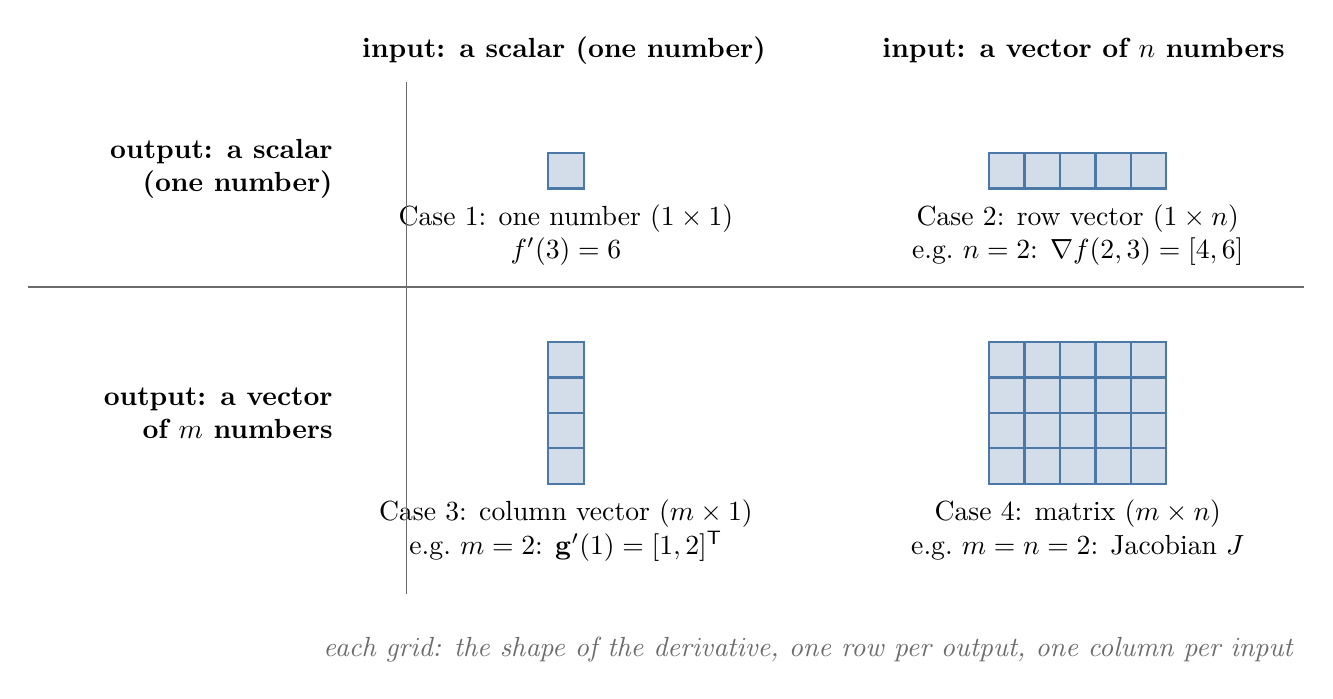
\begin{tikzpicture}
  \node[font=\bfseries] at (2.2,1.3) {input: a scalar (one number)};
  \node[font=\bfseries] at (8.8,1.3) {input: a vector of $n$ numbers};
  \node[font=\bfseries, anchor=east, align=right] at (-0.6,-0.2) {output: a scalar\\ (one number)};
  \node[font=\bfseries, anchor=east, align=right] at (-0.6,-3.3) {output: a vector\\ of $m$ numbers};
  \cell{2}{0}{1}{1}{Case 1: one number ($1 \times 1$)\\ $f'(3) = 6$}
  \cell{7.6}{0}{1}{5}{Case 2: row vector ($1 \times n$)\\ e.g.\ $n = 2$: $\nabla f(2, 3) = [4, 6]$}
  \cell{2}{-2.4}{4}{1}{Case 3: column vector ($m \times 1$)\\ e.g.\ $m = 2$: $\mathbf{g}'(1) = [1, 2]^{\mathsf T}$}
  \cell{7.6}{-2.4}{4}{5}{Case 4: matrix ($m \times n$)\\ e.g.\ $m = n = 2$: Jacobian $J$}
  \draw[cgrey, line width=0.6pt] (0.2,0.9) -- (0.2,-5.6);
  \draw[cgrey, line width=0.6pt] (-4.6,-1.7) -- (11.6,-1.7);
  \node[font=\itshape, cgrey] at (5.3,-6.3) {each grid: the shape of the derivative, one row per output, one column per input};
\end{tikzpicture}
\end{document}
